\documentclass[12pt]{article}

% TEMPLATE DEFAULT PACKAGES
\usepackage{amssymb,amsmath,amsfonts,eurosym,geometry,ulem,graphicx,color,setspace,sectsty,comment,natbib,pdflscape,array,adjustbox}

% ADDED PACKAGES FOR THIS MANUSCRIPT
\usepackage{palatino,newtxmath,multirow,titlesec,threeparttable,tabu,booktabs,titlesec,threeparttable,mathtools,bm,bbm,subcaption,pdflscape,tcolorbox,mathrsfs}
% endfloat,

\usepackage{afterpage}
\usepackage[hyphens]{url}
\usepackage[margin=1cm]{caption}

\usepackage[draft]{hyperref}
\newcommand{\tim}{$\,\times\,$}
% FIGURES & TABLES CAPTION STYLING
\captionsetup[figure]{labelfont={bf},name={Figure},labelsep=period}
\captionsetup[table]{labelfont={bf},name={Table},labelsep=period}

% SECTION TITLE SETTINGS
\titlelabel{\thetitle.\enskip}
\titleformat*{\section}{\large\bfseries}
\titleformat*{\subsection}{\normalsize\bfseries}

% COLUMN TYPES
\newcolumntype{L}[1]{>{\raggedright\let\newline\\\arraybackslash\hspace{0pt}}m{#1}}
\newcolumntype{C}{>{\centering\arraybackslash}p{5.2em}}
\newcolumntype{D}{>{\centering\arraybackslash}p{5em}}
\newcolumntype{R}[1]{>{\raggedleft\let\newline\\\arraybackslash\hspace{0pt}}m{#1}}


% MARGINS AND SPACING
\normalem
\geometry{left=1.1in,right=1.1in,top=1.0in,bottom=1.0in}
\setlength{\parskip}{2.5pt}

% SPECIAL CELL 
\newcommand{\specialcell}[2][c]{%
	\begin{tabular}[#1]{@{}l@{}}#2\end{tabular}}

% NO INDENT ON FOOTNOTES
\usepackage[hang,flushmargin]{footmisc}

\begin{document}



\begin{itemize}

\item raw pre-period building density means show (1) differences between project areas and spillover areas and (2) differences between constructed and unconstructed projects
\item we are going to use two strategies: 
\begin{enumerate}
\item our high-res spatial data provides a unique opportunity to control for spatially precise fixed effects (2001 census subplaces) which erase mean differences between constructed and unconstructed projects in the pre-period and;
\item after controlling for 2001 census subplace fixed effects, constructed and unconstructed projects have the same pattern in the preperiod: both have higher informal building density in project areas, which means it is important to include unconstructed projects as counterfactuals in a DDD setting
\end{enumerate}
	\begin{itemize}
		\item by project type, greenfield and in-situ have perfect pre-trends, while unlabeled projects have a few differences
	\end{itemize}
\item raw building changes over time suggest some crowd-in close to project boundaries, especially for in-situ upgrading projects\footnote{I don't want to show ``demeaned'' changes over time because that is not exactly what the regression is picking up, in fact the regression results are more consistent with the raw changes than the demeaned changes}

\item empirical strategy is a DDD with each observation linked to its closest project and controlling for 2001 census subplace fixed effects
	\begin{itemize}
		\item there are around 1000 sub-places in 2001
		\item using 2001 subplaces is a nice way to tie our hands on geography, and subplaces are likely to be drawn in more thoughtful ways than simply imposing arbitrary 3km grid cells
		% \item the fixed effects results have some differences with the results without fixed effects (in none\_250.pdf), which are consistent with where the identification is coming from (ie. subplaces on the edge of projects so that they are exposed to two treatment conditions, which is probably important to discuss)
		\item specifications define spillover areas as 0-250m and 250-500m distances away from projects
			\begin{itemize}
				\item why 250m?  because the average area of the 250m buffers is just about equal to the average area of the projects themselves (which is 1.2 km2), which is consistent with some rough assumption that spatial effects might be proportional to size of footprint; also, the effects mostly dissipate at further distances
				\footnote{one concern is that there is error in drawing the project boundaries so what we are calling spillover may actually just be mislabeled project areas: three responses
					\begin{itemize}
						\item the raw data show seriously sharp breaks in densities at boundaries
						% \item we find opposite informal density substitution patterns: we find substitution toward bkyd shacks inside projects, but away from bkyd shacks just outside projects 
						\item casual observation suggests that boundaries are often drawn generously (ie. in many cases, houses do not fill the total shapes)
					\end{itemize}}
			\end{itemize}
	\end{itemize}

\item Standard errors are clustered at the project/treatment level (ie. about 300 projects by inside, spillover, and control areas for about 900 groups total).  This approach follows from recommendations from Imbens and Athey's recent paper.  I also tried spatially auto-correlated Conley errors, which are actually a lot smaller than the clustered errors (I don't think you can do these errors on top of clustering), but might be worth reporting also

\item \textbf{My headline takeaways:}
\begin{itemize}
	\item Greenfield projects are characterized by increases in formal housing (with improved services) and backyard informal housing, and small decreases in informal non-bkyd housing.  These new houses slightly crowd-in new formal development (with better services) around their footprints.  New and improved greenfield houses act as a positive amenity, noisily increasing house prices
	\item In-situ projects knock down a lot of informal non-bkyd housing (which is totally offset by new bkyd housing) and replace this informal housing with new formal housing (with improved services).  This big shift in housing quality noisily crowds-in new development of both formal and informal housing (with no strong net effect on services) nearby.  This massive increase in nearby formal housing supply offsets the gain to local amenities and drives down local formal housing prices 
\end{itemize}


\end{itemize}




\vspace{0mm}
\begin{table}[h!]
\centering
\caption{Housing Project Areas Description}\label{table:projectdescriptives}
\vspace{0mm}
\begin{tabular}{l*{1}{cccccc}}
\toprule
  & \multicolumn{2}{c}{\textbf{All}}& \multicolumn{2}{c}{\textbf{Greenfield}}  & \multicolumn{2}{c}{\textbf{In-Situ}}   \\
  &Const. & Unconst. &Const. & Unconst.   & Const. & Unconst. \\
\midrule
 Number of Projects  & 172  & 145  & 43  & 20  & 27  & 29  \\ 
 Area (km2)  & 1.17  & 1.16  & 1.72  & 2.42  & 1.50  & 0.88  \\ 
 Median Construction Yr.  & 2006  & 2006  & 2006  & 2005  & 2004  & 2006  \\ 
 Delivered Houses  & 374  & 11  & 568  & 24  & 702  & 20  \\ 
 House Price in 1 km (R$^\dagger$)  & 188,441  & 218,635  & 194,214  & 186,841  & 179,596  & 208,570  \\ 
 Distance to CBD$^\ddagger$ (km)  & 32.5  & 27.7  & 40.5  & 39.9  & 32.6  & 30.6  \\ 

\bottomrule
\multicolumn{7}{l}{\scriptsize Const. refers to constructed projects and unconst. refers to unconstructed projects.}\\[-.5em]
\multicolumn{7}{l}{\scriptsize $^*$Calculated from {\it expected} completion dates using Gauteng National Treasury budget reports.}\\[-.5em]
\multicolumn{7}{l}{\scriptsize $^\dagger$ The USD averaged to about 7.70 Rands during the 2001-2011 period.}\\[-.5em]
\multicolumn{7}{l}{\scriptsize $^\ddagger$Measured as the average minimum distance with respect to Johannesburg and Pretoria CBDs. } \\[-.5em]
%\multicolumn{7}{l}{\scriptsize City includes projects whose centroids are within 30.4 km of their nearest CBD.} \\[-.5em]
%\multicolumn{7}{l}{\scriptsize Suburb includes projects whose centroids are further than 30.4 km from their nearest CBD.}
\end{tabular}
\end{table} 




% \vspace{0mm}
% \begin{table}[h!]
% \centering
% \caption{Housing Project Areas Description}\label{table:projectdescriptives}
% \vspace{0mm}
% \begin{tabular}{l*{1}{cccccc}}
% \toprule
%   & \multicolumn{2}{c}{\textbf{All}}& \multicolumn{2}{c}{\textbf{Greenfield}}  & \multicolumn{2}{c}{\textbf{In-Situ}}   \\
%   &Const. & Unconst. &Const. & Unconst.   & Const. & Unconst. \\
% \midrule
%  Number of Projects  & 172  & 145  & 43  & 20  & 27  & 29  \\ 
 Area (km2)  & 1.17  & 1.16  & 1.72  & 2.42  & 1.50  & 0.88  \\ 
 Median Construction Yr.  & 2006  & 2006  & 2006  & 2005  & 2004  & 2006  \\ 
 Delivered Houses  & 374  & 11  & 568  & 24  & 702  & 20  \\ 
 House Price in 1 km (R$^\dagger$)  & 188,441  & 218,635  & 194,214  & 186,841  & 179,596  & 208,570  \\ 
 Distance to CBD$^\ddagger$ (km)  & 32.5  & 27.7  & 40.5  & 39.9  & 32.6  & 30.6  \\ 

% \bottomrule
% \multicolumn{7}{l}{\scriptsize Const. refers to constructed projects and unconst. refers to unconstructed projects.}\\[-.5em]
% \multicolumn{7}{l}{\scriptsize $^*$Calculated from {\it expected} completion dates using Gauteng National Treasury budget reports.}\\[-.5em]
% \multicolumn{7}{l}{\scriptsize $^\dagger$ The USD averaged to about 7.70 Rands during the 2001-2011 period.}\\[-.5em]
% \multicolumn{7}{l}{\scriptsize $^\ddagger$Measured as the average minimum distance with respect to Johannesburg and Pretoria CBDs. } \\[-.5em]
% %\multicolumn{7}{l}{\scriptsize City includes projects whose centroids are within 30.4 km of their nearest CBD.} \\[-.5em]
% %\multicolumn{7}{l}{\scriptsize Suburb includes projects whose centroids are further than 30.4 km from their nearest CBD.}
% \end{tabular}
% \end{table} 



\begin{figure*}
        \centering
   %     \caption[ Pre-Period Housing Densities in Constructed and Unconstructed Projects Areas ]
  %      {\small Pre-Period Densities} 
        %\vspace{2mm}
        \begin{subfigure}[b]{0.48\textwidth}
                    \caption[Network2]%
            {{\footnotesize \textbf{All Projects} pre-period formal raw data}}    
            \label{fig:prefor}
            \centering
            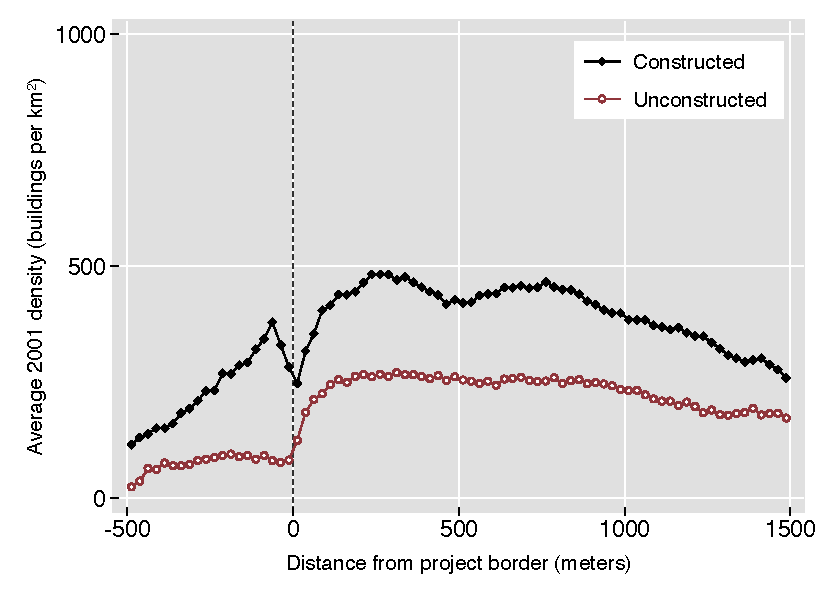
\includegraphics[width=\textwidth,trim={0.3cm .3cm 0.1cm 0cm}, clip=true]{figures/bblu_for_pre_means_4_spk.pdf}

        \end{subfigure}
        \hfill
        \begin{subfigure}[b]{0.48\textwidth}  
                    \caption[]%
            {{\footnotesize \textbf{All Projects} pre-period informal  raw data}}      
            \label{fig:preinf}
            \centering 
            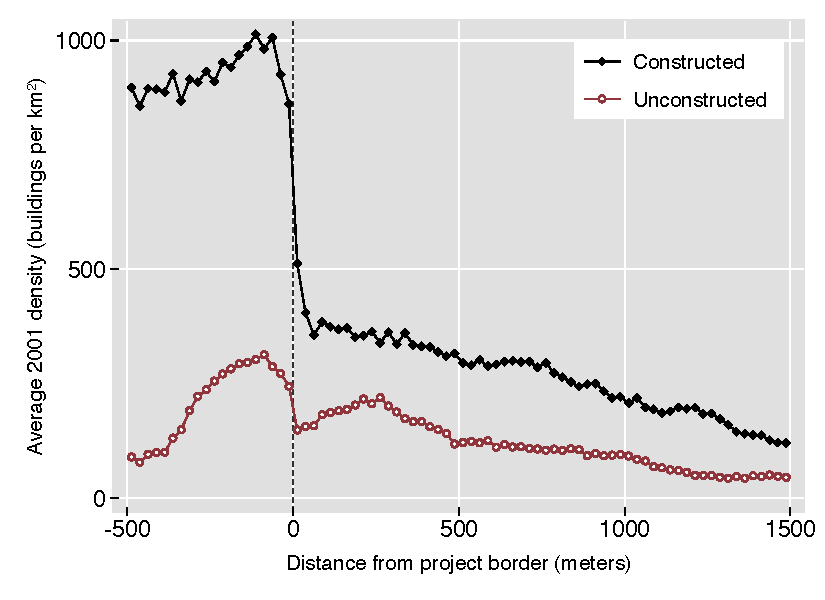
\includegraphics[width=\textwidth,trim={0.3cm .3cm 0.1cm 0cm}, clip=true]{figures/bblu_inf_pre_means_4_spk.pdf}

        \end{subfigure}
        \begin{subfigure}[b]{0.48\textwidth}
                    \caption[Network2]%
            {{\footnotesize \textbf{Greenfield} pre-period formal  raw data}}    
            \label{fig:prefor}
            \centering
            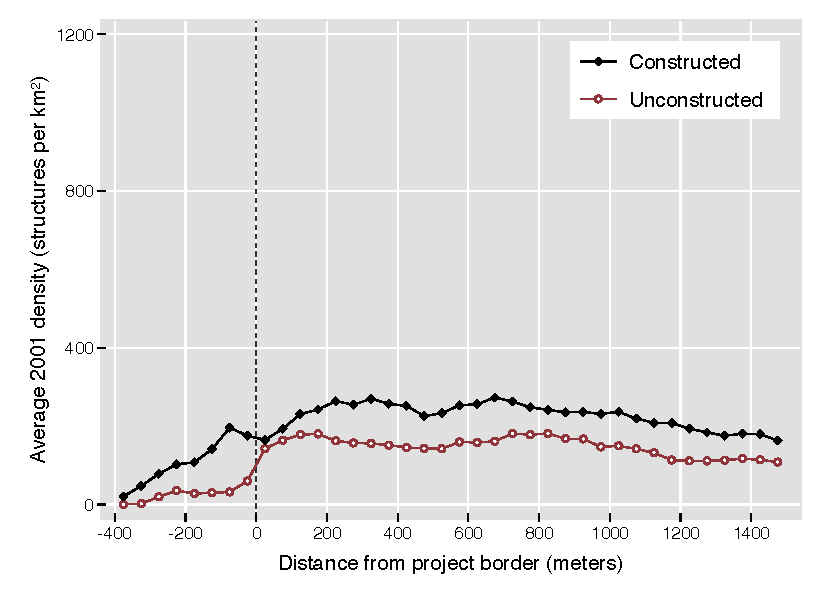
\includegraphics[width=\textwidth,trim={0.3cm .3cm 0.1cm 0cm}, clip=true]{figures/bblu_for_pre_means_4_1_spk.pdf}

        \end{subfigure}
        \hfill
        \begin{subfigure}[b]{0.48\textwidth}  
                    \caption[]%
            {{\footnotesize \textbf{Greenfield} pre-period informal  raw data}}     
            \label{fig:preinf}
            \centering 
            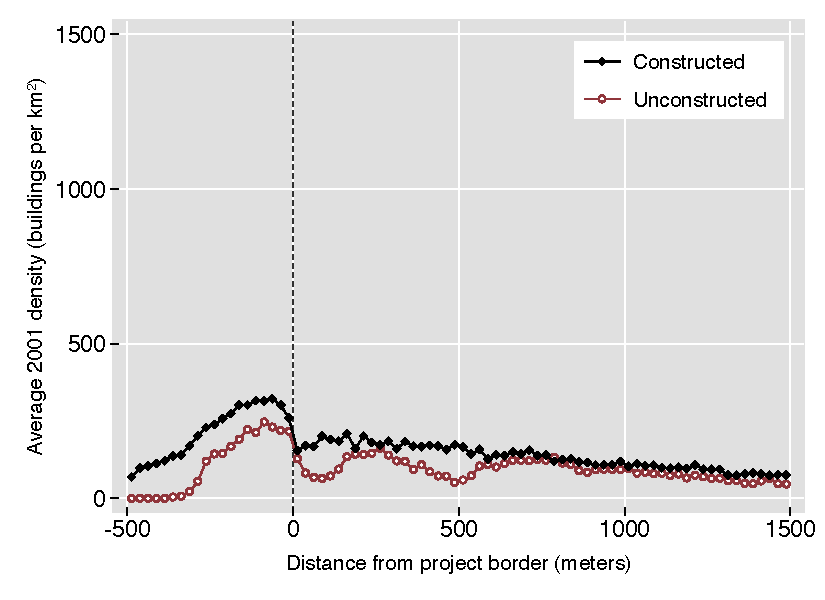
\includegraphics[width=\textwidth,trim={0.3cm .3cm 0.1cm 0cm}, clip=true]{figures/bblu_inf_pre_means_4_1_spk.pdf}

        \end{subfigure}
        \begin{subfigure}[b]{0.48\textwidth}
                    \caption[Network2]%
            {{\footnotesize \textbf{In-Situ} pre-period formal  raw data}}   
            \label{fig:prefor}
            \centering
            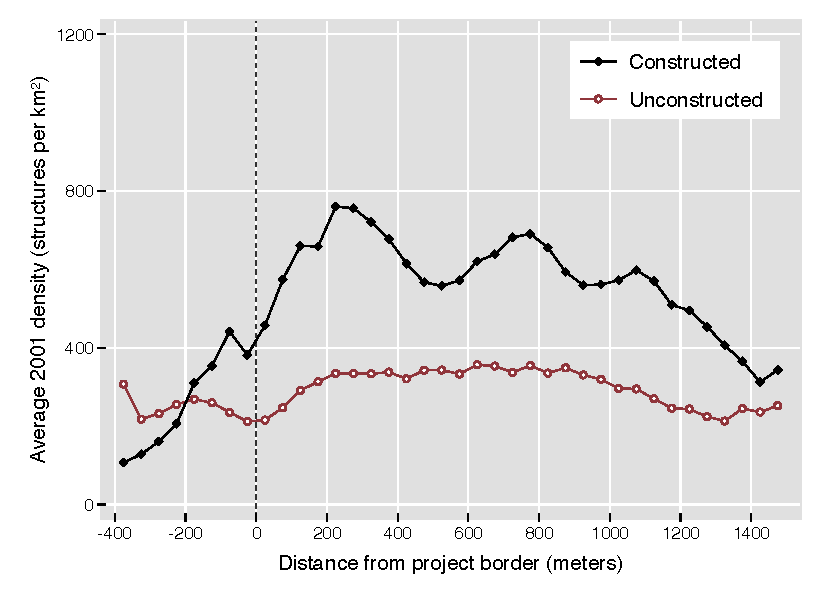
\includegraphics[width=\textwidth,trim={0.3cm .3cm 0.1cm 0cm}, clip=true]{figures/bblu_for_pre_means_4_2_spk.pdf}

        \end{subfigure}
        \hfill
        \begin{subfigure}[b]{0.48\textwidth}  
                    \caption[]%
            {{\footnotesize \textbf{In-Situ} pre-period informal  raw data}}     
            \label{fig:preinf}
            \centering 
            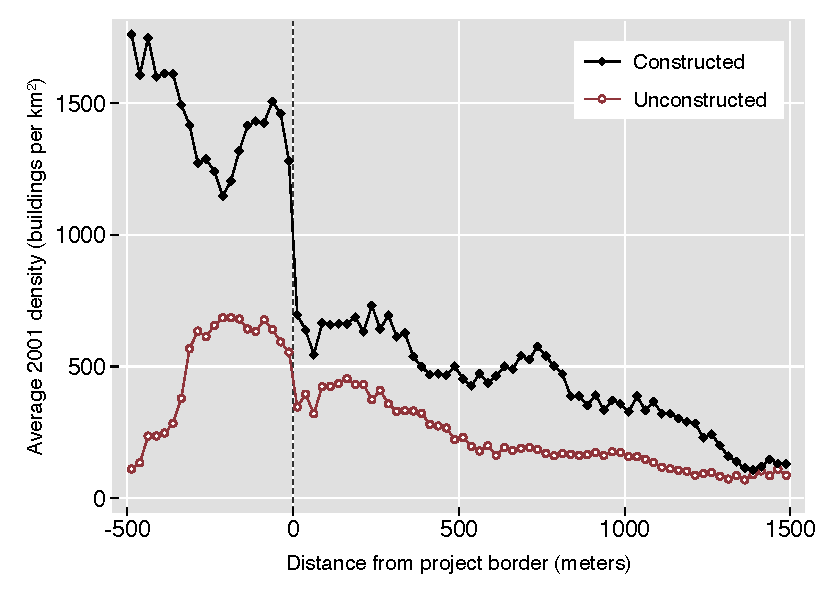
\includegraphics[width=\textwidth,trim={0.3cm .3cm 0.1cm 0cm}, clip=true]{figures/bblu_inf_pre_means_4_2_spk.pdf}

        \end{subfigure}
        \begin{subfigure}[b]{0.48\textwidth}
                    \caption[Network2]%
            {{\footnotesize \textbf{Other} pre-period formal  raw data}}   
            \label{fig:prefor}
            \centering
            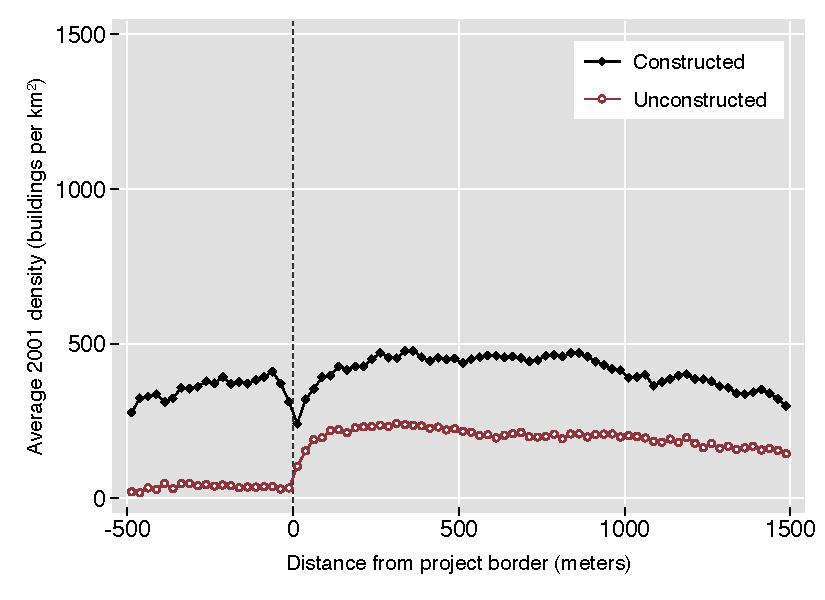
\includegraphics[width=\textwidth,trim={0.3cm .3cm 0.1cm 0cm}, clip=true]{figures/bblu_for_pre_means_4_3_spk.pdf}

        \end{subfigure}
        \hfill
        \begin{subfigure}[b]{0.48\textwidth}  
                    \caption[]%
            {{\footnotesize \textbf{Other} pre-period informal  raw data}}      
            \label{fig:preinf}
            \centering 
            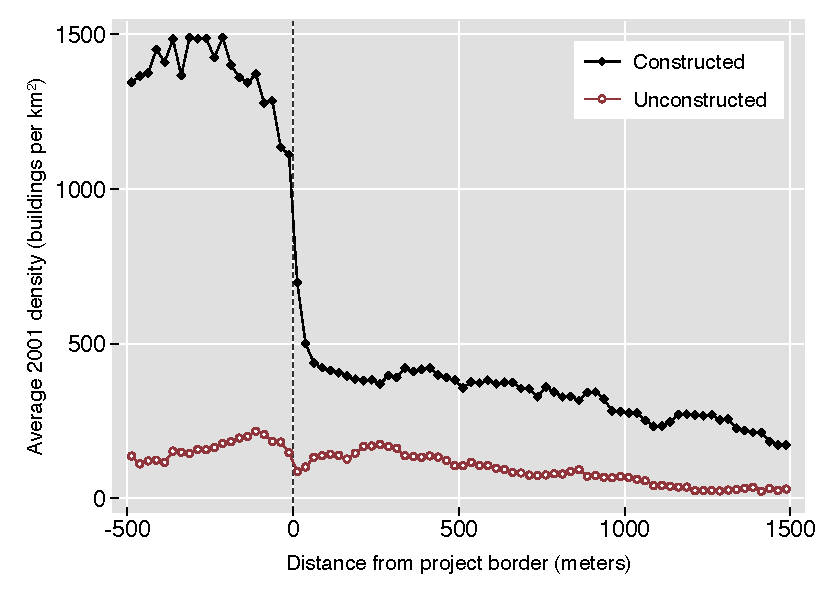
\includegraphics[width=\textwidth,trim={0.3cm .3cm 0.1cm 0cm}, clip=true]{figures/bblu_inf_pre_means_4_3_spk.pdf}

        \end{subfigure}
\end{figure*}




\begin{figure*}
        \centering
   %     \caption[ Pre-Period Housing Densities in Constructed and Unconstructed Projects Areas ]
  %      {\small Pre-Period Densities} 
        %\vspace{2mm}
        \begin{subfigure}[b]{0.48\textwidth}
                    \caption[Network2]%
            {{\footnotesize \textbf{All Projects} pre-period formal fe}}    
            \label{fig:prefor}
            \centering
            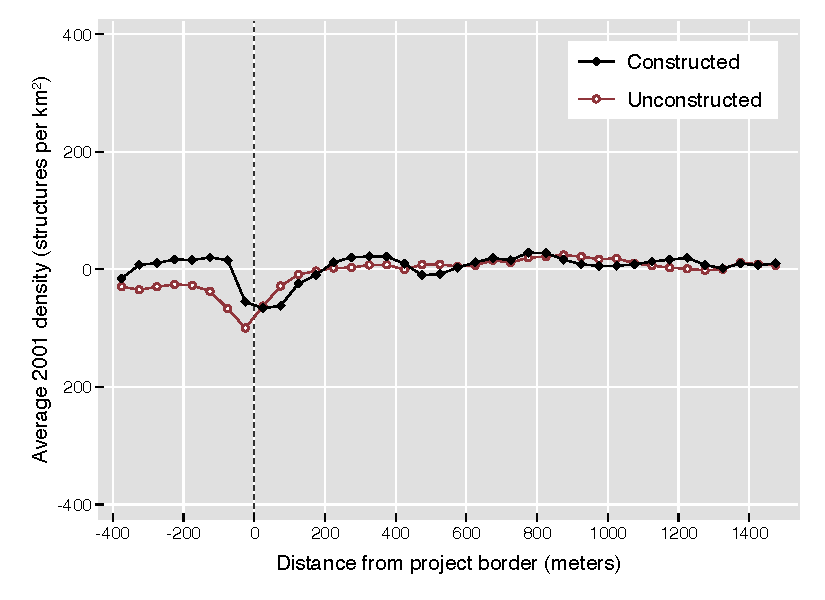
\includegraphics[width=\textwidth,trim={0.3cm .3cm 0.1cm 0cm}, clip=true]{figures/bblu_for_fe_pre_means_4_sp_postk.pdf}

        \end{subfigure}
        \hfill
        \begin{subfigure}[b]{0.48\textwidth}  
                    \caption[]%
            {{\footnotesize \textbf{All Projects} pre-period informal fe }}      
            \label{fig:preinf}
            \centering 
            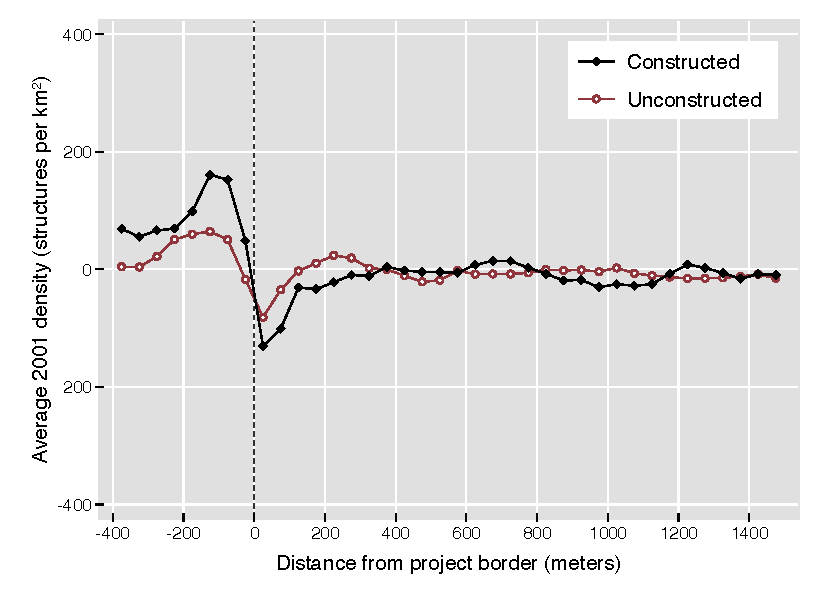
\includegraphics[width=\textwidth,trim={0.3cm .3cm 0.1cm 0cm}, clip=true]{figures/bblu_inf_fe_pre_means_4_sp_postk.pdf}

        \end{subfigure}
        \begin{subfigure}[b]{0.48\textwidth}
                    \caption[Network2]%
            {{\footnotesize \textbf{Greenfield} pre-period formal  fe }}    
            \label{fig:prefor}
            \centering
            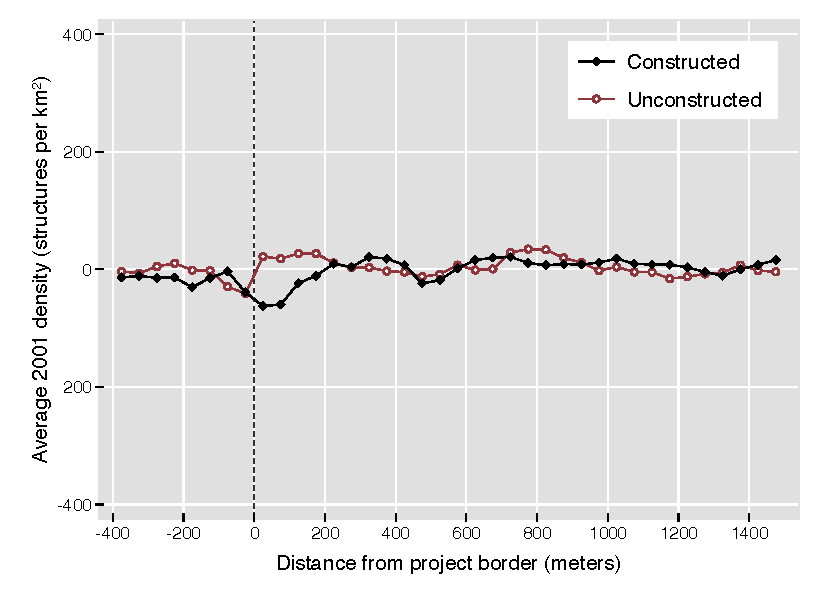
\includegraphics[width=\textwidth,trim={0.3cm .3cm 0.1cm 0cm}, clip=true]{figures/bblu_for_fe_pre_means_4_1_sp_postk.pdf}

        \end{subfigure}
        \hfill
        \begin{subfigure}[b]{0.48\textwidth}  
                    \caption[]%
            {{\footnotesize \textbf{Greenfield} pre-period informal fe }}     
            \label{fig:preinf}
            \centering 
            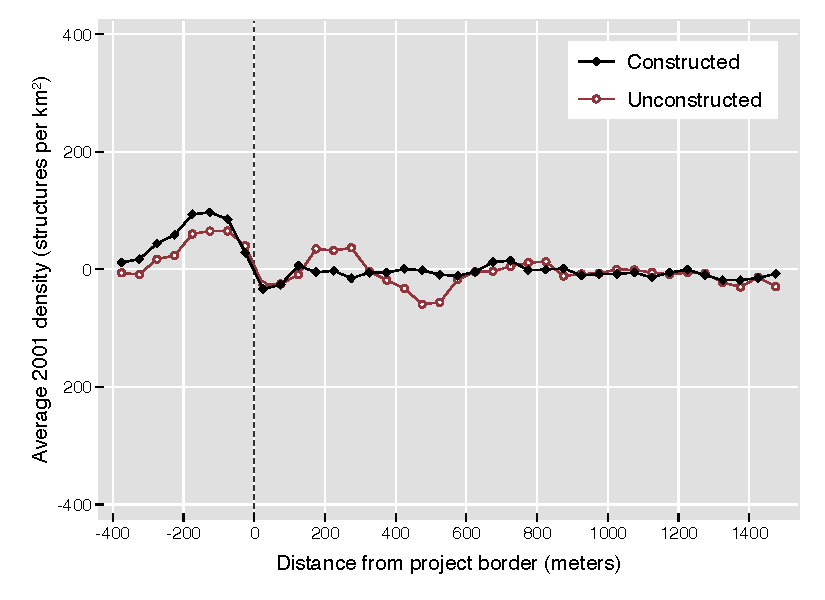
\includegraphics[width=\textwidth,trim={0.3cm .3cm 0.1cm 0cm}, clip=true]{figures/bblu_inf_fe_pre_means_4_1_sp_postk.pdf}

        \end{subfigure}
        \begin{subfigure}[b]{0.48\textwidth}
                    \caption[Network2]%
            {{\footnotesize \textbf{In-Situ} pre-period formal fe }}   
            \label{fig:prefor}
            \centering
            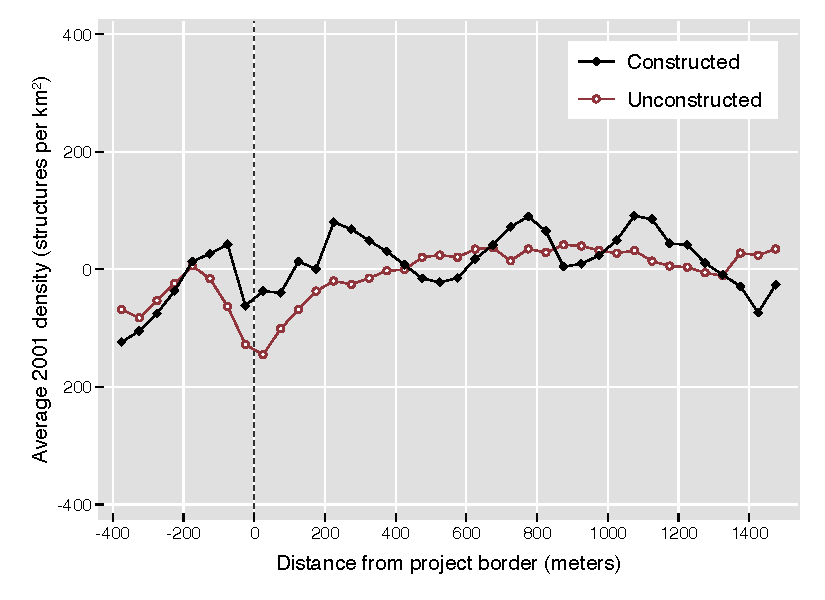
\includegraphics[width=\textwidth,trim={0.3cm .3cm 0.1cm 0cm}, clip=true]{figures/bblu_for_fe_pre_means_4_2_sp_postk.pdf}

        \end{subfigure}
        \hfill
        \begin{subfigure}[b]{0.48\textwidth}  
                    \caption[]%
            {{\footnotesize \textbf{In-Situ} pre-period informal fe }}     
            \label{fig:preinf}
            \centering 
            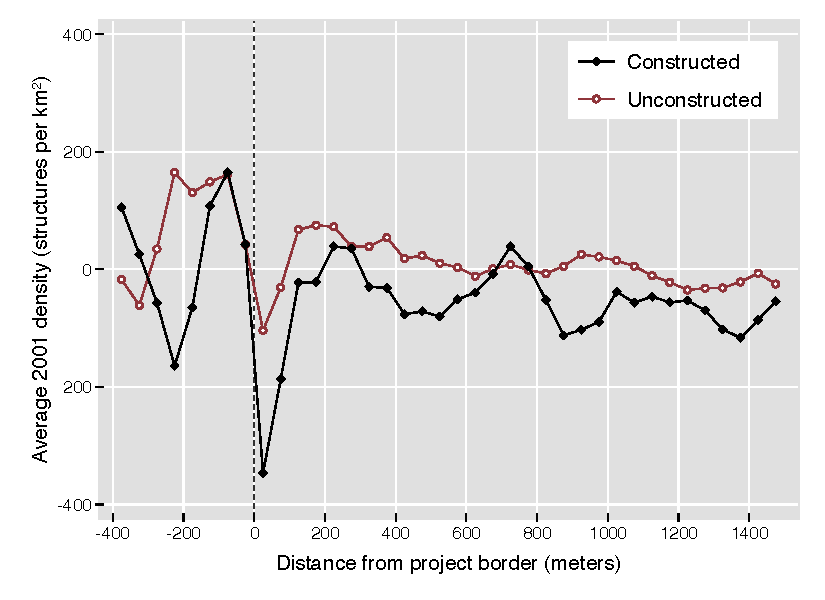
\includegraphics[width=\textwidth,trim={0.3cm .3cm 0.1cm 0cm}, clip=true]{figures/bblu_inf_fe_pre_means_4_2_sp_postk.pdf}

        \end{subfigure}
        \begin{subfigure}[b]{0.48\textwidth}
                    \caption[Network2]%
            {{\footnotesize \textbf{Other} pre-period formal fe }}   
            \label{fig:prefor}
            \centering
            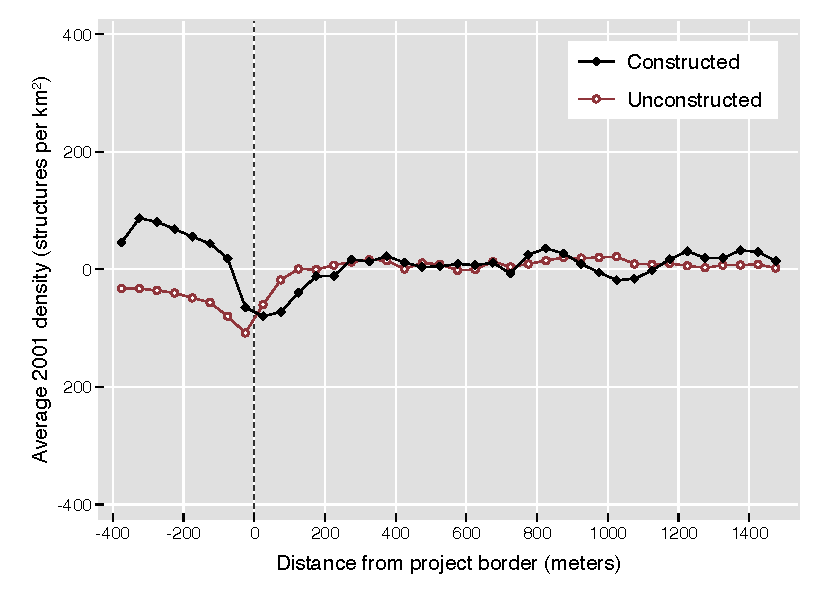
\includegraphics[width=\textwidth,trim={0.3cm .3cm 0.1cm 0cm}, clip=true]{figures/bblu_for_fe_pre_means_4_3_sp_postk.pdf}

        \end{subfigure}
        \hfill
        \begin{subfigure}[b]{0.48\textwidth}  
                    \caption[]%
            {{\footnotesize \textbf{Other} pre-period informal fe }}      
            \label{fig:preinf}
            \centering 
            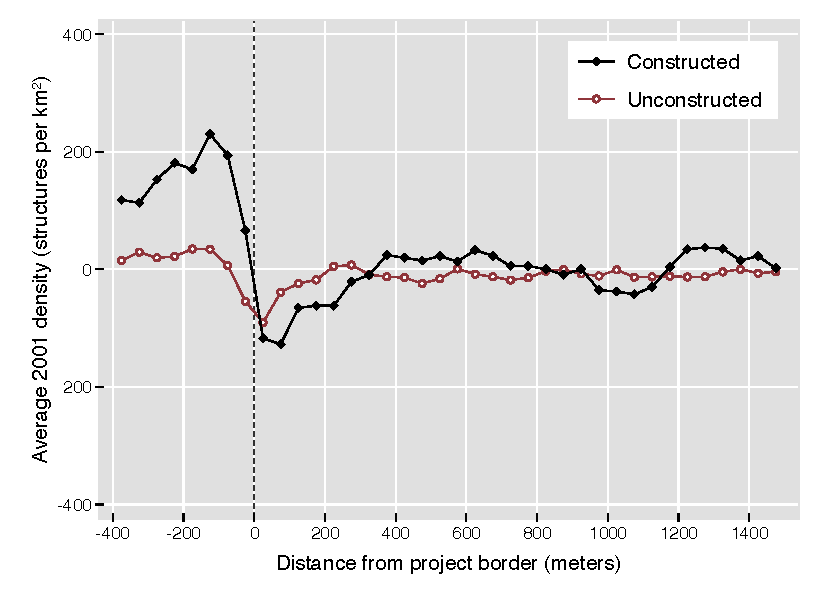
\includegraphics[width=\textwidth,trim={0.3cm .3cm 0.1cm 0cm}, clip=true]{figures/bblu_inf_fe_pre_means_4_3_sp_postk.pdf}

        \end{subfigure}
\end{figure*}









\begin{figure*}
        \centering
   %     \caption[ Pre-Period Housing Densities in Constructed and Unconstructed Projects Areas ]
  %      {\small Pre-Period Densities} 
        %\vspace{2mm}
        \begin{subfigure}[b]{0.48\textwidth}
            \caption[Network2]%
            {{\footnotesize \textbf{All Projects} changes formal raw data}}    
            \label{fig:prefor}
            \centering
            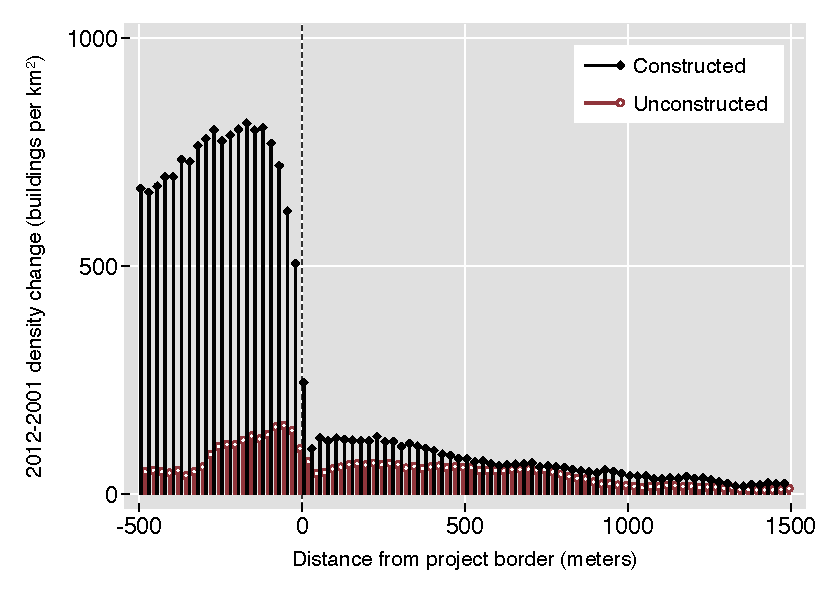
\includegraphics[width=\textwidth,trim={0.3cm .3cm 0.1cm 0cm}, clip=true]{figures/bblu_for_rawchanges_4_spk.pdf}

        \end{subfigure}
        \hfill
        \begin{subfigure}[b]{0.48\textwidth}  
                    \caption[]%
            {{\footnotesize \textbf{All Projects} changes informal  raw data}}      
            \label{fig:preinf}
            \centering 
            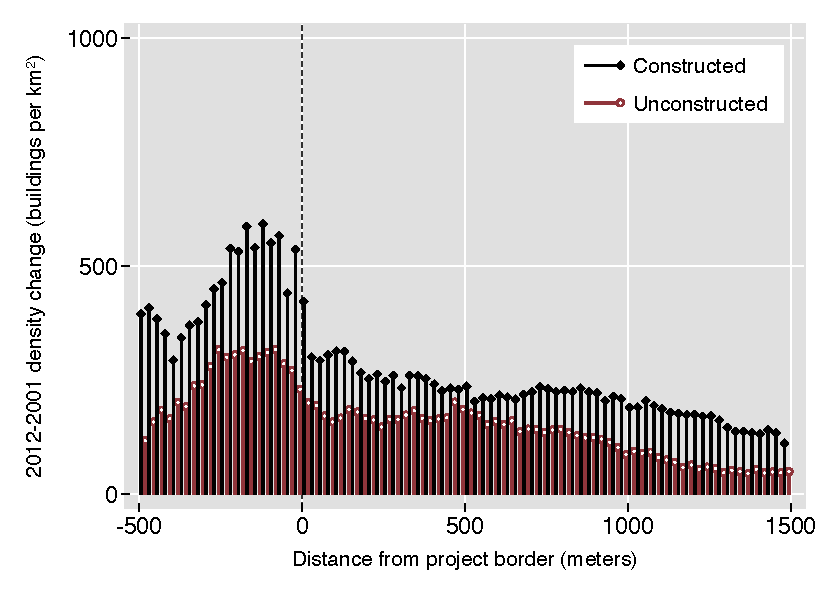
\includegraphics[width=\textwidth,trim={0.3cm .3cm 0.1cm 0cm}, clip=true]{figures/bblu_inf_rawchanges_4_spk.pdf}

        \end{subfigure}
        \begin{subfigure}[b]{0.48\textwidth}
                    \caption[Network2]%
            {{\footnotesize \textbf{Greenfield} changes formal  raw data}}    
            \label{fig:prefor}
            \centering
            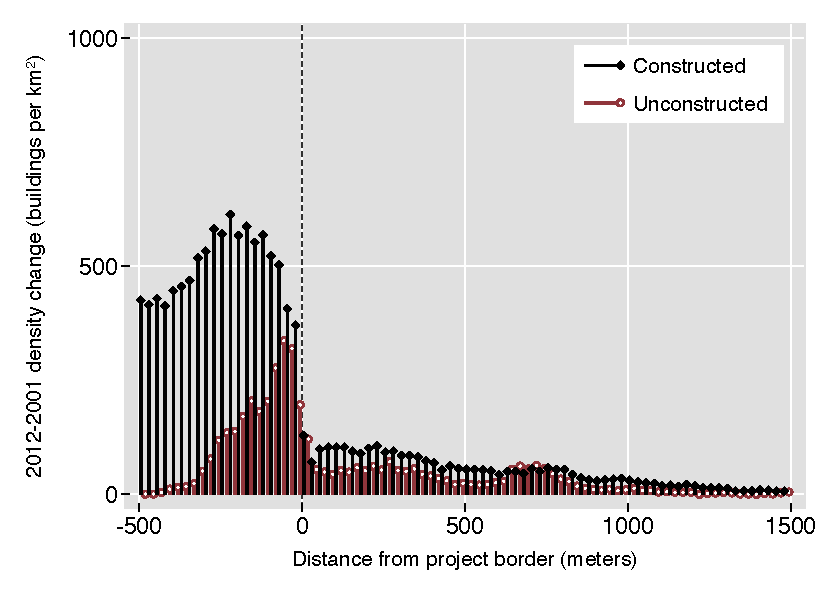
\includegraphics[width=\textwidth,trim={0.3cm .3cm 0.1cm 0cm}, clip=true]{figures/bblu_for_rawchanges_4_1_spk.pdf}

        \end{subfigure}
        \hfill
        \begin{subfigure}[b]{0.48\textwidth}  
                    \caption[]%
            {{\footnotesize \textbf{Greenfield} changes informal raw data }}     
            \label{fig:preinf}
            \centering 
            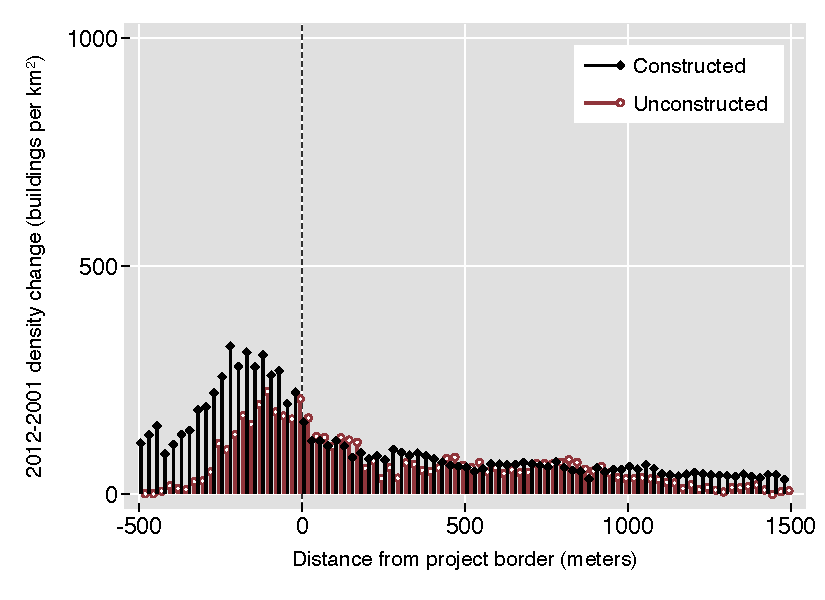
\includegraphics[width=\textwidth,trim={0.3cm .3cm 0.1cm 0cm}, clip=true]{figures/bblu_inf_rawchanges_4_1_spk.pdf}

        \end{subfigure}
        \begin{subfigure}[b]{0.48\textwidth}
                    \caption[Network2]%
            {{\footnotesize \textbf{In-Situ} changes formal raw data }}   
            \label{fig:prefor}
            \centering
            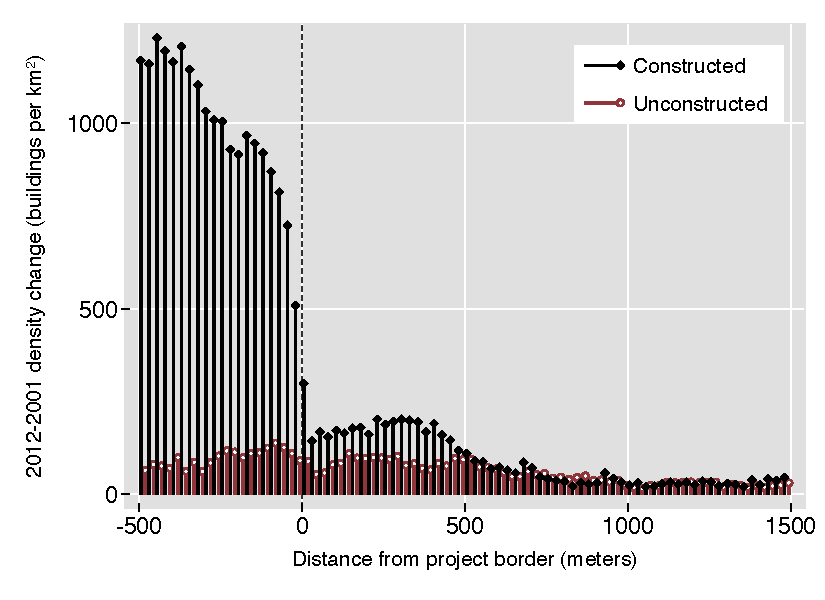
\includegraphics[width=\textwidth,trim={0.3cm .3cm 0.1cm 0cm}, clip=true]{figures/bblu_for_rawchanges_4_2_spk.pdf}

        \end{subfigure}
        \hfill
        \begin{subfigure}[b]{0.48\textwidth}  
                    \caption[]%
            {{\footnotesize \textbf{In-Situ} changes informal raw data }}     
            \label{fig:preinf}
            \centering 
            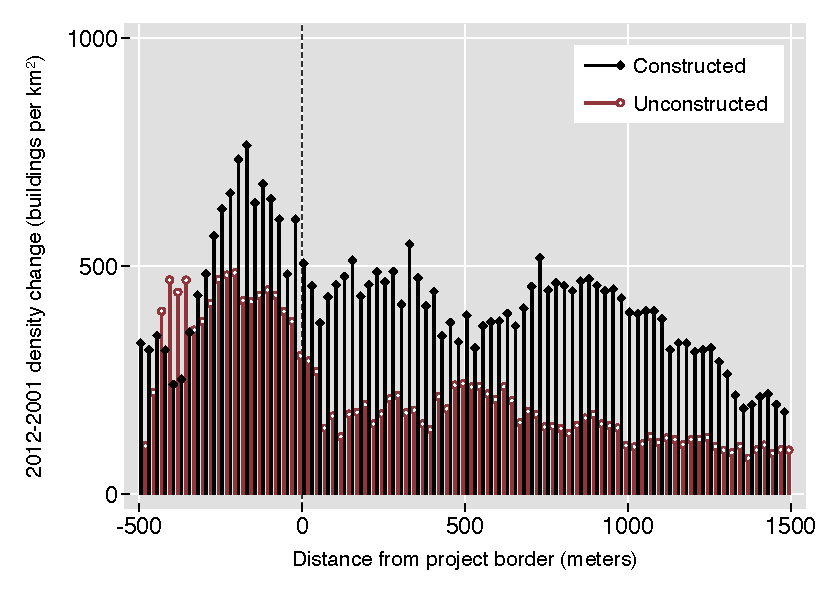
\includegraphics[width=\textwidth,trim={0.3cm .3cm 0.1cm 0cm}, clip=true]{figures/bblu_inf_rawchanges_4_2_spk.pdf}

        \end{subfigure}
        \begin{subfigure}[b]{0.48\textwidth}
                    \caption[Network2]%
            {{\footnotesize \textbf{Other} changes formal raw data}}   
            \label{fig:prefor}
            \centering
            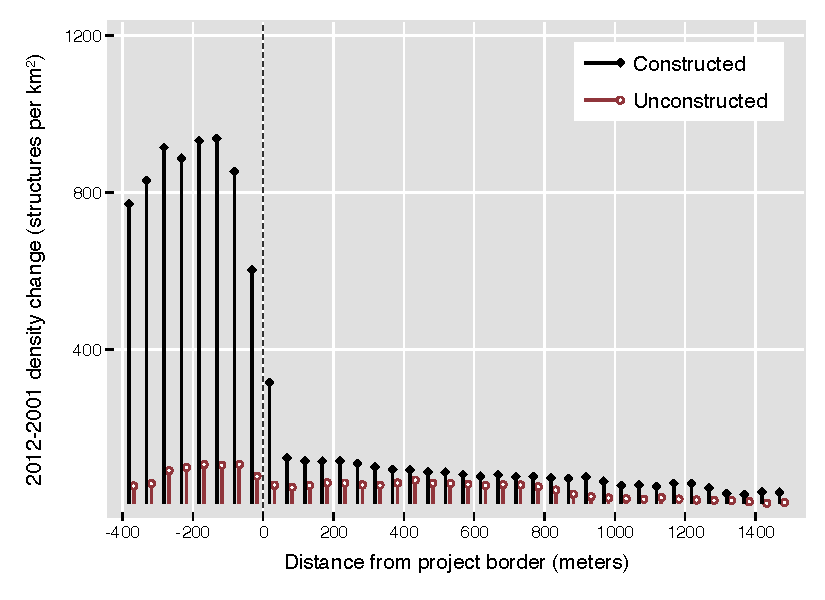
\includegraphics[width=\textwidth,trim={0.3cm .3cm 0.1cm 0cm}, clip=true]{figures/bblu_for_rawchanges_4_3_spk.pdf}

        \end{subfigure}
        \hfill
        \begin{subfigure}[b]{0.48\textwidth} 
                    \caption[]%
            {{\footnotesize \textbf{Other} changes informal  raw data}}      
            \label{fig:preinf} 
            \centering 
            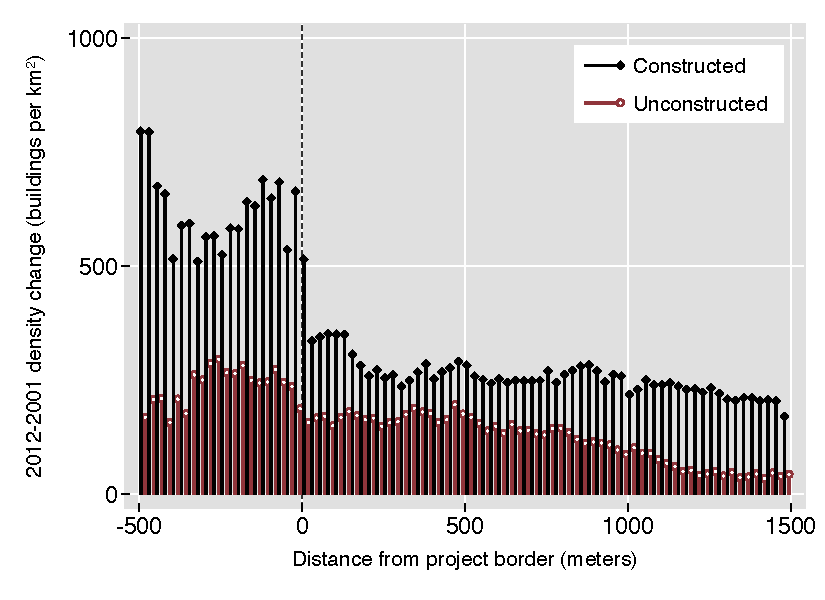
\includegraphics[width=\textwidth,trim={0.3cm .3cm 0.1cm 0cm}, clip=true]{figures/bblu_inf_rawchanges_4_3_spk.pdf}

        \end{subfigure}
\end{figure*}







\begin{table}
\caption{Building Density}
\begin{tabular}{lDDDDD}
\toprule
 & \small (1) & \small (2)  & \small (3) & \small (4) & \small (5) \\
 & Total & Formal  & Informal & Informal Bkyd. & Informal Non-Bkyd. \\ \midrule
\textbf{All Projects} \\inside project      &     788.743\textsuperscript{a}&     619.987\textsuperscript{a}&     168.756\textsuperscript{c}&     570.667\textsuperscript{a}&    -401.911\textsuperscript{a}\\
                    &   (147.153)                   &    (74.706)                   &   (102.449)                   &   (107.185)                   &    (81.969)                   \\[0.5em]
0-400m outside project &      56.801                   &      49.969\textsuperscript{b}&       6.831                   &      53.785                   &     -46.954                   \\
                    &    (61.195)                   &    (24.770)                   &    (52.301)                   &    (48.041)                   &    (29.618)                   \\[0.5em]
400-800m outside project &     -37.033                   &      -1.117                   &     -35.916                   &       0.511                   &     -36.426\textsuperscript{b}\\
                    &    (58.925)                   &    (22.007)                   &    (48.977)                   &    (45.711)                   &    (18.128)                   \\[0.5em]
R$^2$               &       0.422                   &       0.394                   &       0.378                   &       0.329                   &       0.325                   \\

\midrule
\textbf{Greenfield} \\   inside project      &     560.424\textsuperscript{a}&     415.686\textsuperscript{a}&     144.738\textsuperscript{c}&     231.966\textsuperscript{b}&     -87.228                   \\
                    &   (199.447)                   &   (137.150)                   &    (85.455)                   &   (105.735)                   &    (58.891)                   \\[0.01em]
0-400m outside project &      40.680                   &      30.986                   &       9.694                   &       7.684                   &       2.010                   \\
                    &    (66.572)                   &    (34.200)                   &    (45.871)                   &    (44.640)                   &    (36.235)                   \\[0.01em]
400-800m outside project &      10.437                   &      10.479                   &      -0.042                   &      10.630                   &     -10.672                   \\
                    &    (55.404)                   &    (27.839)                   &    (37.650)                   &    (31.294)                   &    (20.001)                   \\[0.8em] 
\textbf{In-Situ Upgrading} \\   inside project      &     765.421\textsuperscript{b}&     837.504\textsuperscript{a}&     -72.083                   &     769.575\textsuperscript{a}&    -841.658\textsuperscript{a}\\
                    &   (373.403)                   &   (149.353)                   &   (307.415)                   &   (276.283)                   &   (226.921)                   \\[0.01em]
0-400m outside project &     155.396                   &     102.399                   &      52.997                   &     111.880                   &     -58.883                   \\
                    &   (180.360)                   &    (90.121)                   &   (167.551)                   &   (150.951)                   &   (115.929)                   \\[0.01em]
400-800m outside project &      -6.638                   &      16.872                   &     -23.510                   &      -3.809                   &     -19.700                   \\
                    &   (162.416)                   &    (43.786)                   &   (151.370)                   &   (136.792)                   &    (64.367)                   \\[0.8em]
\textbf{Other} \\   inside project      &     947.010\textsuperscript{a}&     691.162\textsuperscript{a}&     255.848\textsuperscript{c}&     708.920\textsuperscript{a}&    -453.072\textsuperscript{a}\\
                    &   (178.270)                   &    (76.300)                   &   (145.328)                   &   (126.026)                   &   (101.600)                   \\[0.01em]
0-400m outside project &      16.626                   &      43.432                   &     -26.805                   &      39.404                   &     -66.209\textsuperscript{c}\\
                    &    (88.300)                   &    (31.582)                   &    (76.650)                   &    (68.551)                   &    (37.427)                   \\[0.01em]
400-800m outside project &     -75.515                   &     -11.115                   &     -64.400                   &      -6.287                   &     -58.113\textsuperscript{b}\\
                    &    (87.097)                   &    (37.431)                   &    (72.029)                   &    (68.283)                   &    (27.257)                   \\[0.8em]
Mean Outcome 2001   &      526.22                   &      261.56                   &      264.66                   &       96.43                   &      168.23                   \\
Mean Outcome 2011   &      838.62                   &      385.14                   &      453.48                   &      286.79                   &      166.69                   \\
R$^2$               &       0.425                   &       0.396                   &       0.381                   &       0.336                   &       0.327                   \\
N                   &   1,705,534                   &   1,705,534                   &   1,705,534                   &   1,705,534                   &   1,705,534                   \\

\bottomrule
\end{tabular}
\end{table}





\begin{table}
\caption{Building Density Two Diff-in-Diffs}
\begin{tabular}{lDDDDD}
\toprule
 & \small (1) & \small (2)  & \small (3) & \small (4) & \small (5) \\
 & Total & Formal  & Informal & Informal Bkyd. & Informal Non-Bkyd. \\ \midrule
\textbf{Constructed} \\ inside project      &     953.625\textsuperscript{a}&     697.412\textsuperscript{a}&     256.213\textsuperscript{a}&     538.576\textsuperscript{a}&    -282.363\textsuperscript{a}\\
                    &   (137.091)                   &    (81.827)                   &    (82.762)                   &   (109.884)                   &    (77.540)                   \\[0.5em]
0-400m outside project &     266.683\textsuperscript{a}&     139.368\textsuperscript{a}&     127.314\textsuperscript{a}&     149.380\textsuperscript{a}&     -22.066                   \\
                    &    (50.493)                   &    (21.453)                   &    (42.545)                   &    (39.721)                   &    (25.696)                   \\[0.5em]
400-800m outside project &     215.834\textsuperscript{a}&     121.526\textsuperscript{a}&      94.308\textsuperscript{b}&     132.293\textsuperscript{a}&     -37.986\textsuperscript{c}\\
                    &    (47.239)                   &    (17.930)                   &    (40.692)                   &    (36.409)                   &    (22.150)                   \\[0.5em]
\textbf{Unconstructed} \\ inside project      &     340.832\textsuperscript{a}&      72.801                   &     268.031\textsuperscript{b}&      13.700                   &     254.331\textsuperscript{b}\\
                    &   (129.753)                   &    (49.891)                   &   (110.918)                   &    (54.821)                   &   (105.493)                   \\[0.5em]
0-400m outside project &     377.616\textsuperscript{a}&     142.894\textsuperscript{a}&     234.722\textsuperscript{a}&     223.610\textsuperscript{a}&      11.112                   \\
                    &    (73.168)                   &    (42.464)                   &    (58.995)                   &    (52.787)                   &    (46.823)                   \\[0.5em]
400-800m outside project &     483.917\textsuperscript{a}&     181.762\textsuperscript{a}&     302.155\textsuperscript{a}&     247.238\textsuperscript{a}&      54.917                   \\
                    &    (79.678)                   &    (45.102)                   &    (68.963)                   &    (53.623)                   &    (69.973)                   \\[0.5em]
R$^2$               &       0.420                   &       0.391                   &       0.376                   &       0.326                   &       0.323                   \\

\midrule
\textbf{Treatment} \\ inside project      &     683.341\textsuperscript{a}&     631.009\textsuperscript{a}&      52.333                   &     605.043\textsuperscript{a}&    -552.710\textsuperscript{a}\\
                    &   (185.134)                   &    (95.077)                   &   (134.702)                   &   (119.221)                   &   (130.455)                   \\[0.5em]
0-400m outside project &     -40.650                   &       2.821                   &     -43.471                   &       5.728                   &     -49.199                   \\
                    &    (80.954)                   &    (46.035)                   &    (65.476)                   &    (59.177)                   &    (52.262)                   \\[0.5em]
400-800m outside project &    -191.871\textsuperscript{b}&     -52.804                   &    -139.067\textsuperscript{c}&     -30.101                   &    -108.966                   \\
                    &    (84.293)                   &    (46.846)                   &    (72.922)                   &    (57.117)                   &    (72.423)                   \\[0.5em]
\textbf{Control} \\ 800-1500m outside project&      69.778\textsuperscript{c}&       4.663                   &      65.115\textsuperscript{b}&      78.877\textsuperscript{a}&     -13.762                   \\
                    &    (37.298)                   &    (12.234)                   &    (32.181)                   &    (29.897)                   &    (11.195)                   \\[0.5em]
R$^2$               &       0.420                   &       0.391                   &       0.376                   &       0.326                   &       0.323                   \\

\bottomrule
\end{tabular}
\end{table}









% \begin{table}[]
% \small
% \centering
% \caption{Census Household-level Estimates }\label{table:censusestimates}
% \vspace{-2mm}
% \resizebox{.9\linewidth}{!}{
% \begin{tabular}{lDDDDD}
% \toprule
%  & \small (1) & \small (2)  & \small (3) & \small (4) & \small (5)  \\
% & \small Formal Bkyd  & \small Formal Non-Bkyd & \small Informal Bkyd& Informal Non-Bkyd  & \small Own Dwelling \\ \midrule 
% \textbf{All Projects} \\inside project      &       0.483\textsuperscript{a}&      -0.451\textsuperscript{a}&      -0.089                   \\
                    &     (0.076)                   &     (0.076)                   &     (0.081)                   \\[0.5em]
0-250m outside project &       0.011                   &       0.032                   &       0.044                   \\
                    &     (0.065)                   &     (0.060)                   &     (0.057)                   \\[0.5em]
250-500m outside project &       0.011                   &      -0.058                   &       0.012                   \\
                    &     (0.064)                   &     (0.056)                   &     (0.059)                   \\[0.5em]
R$^2$               &       0.519                   &       0.586                   &       0.427                   \\

% \midrule
% \textbf{Greenfield} \\   inside project      &       0.309\textsuperscript{a}&      -0.243\textsuperscript{a}&      -0.048                   \\
                    &     (0.088)                   &     (0.090)                   &     (0.087)                   \\[0.01em]
0-250m outside project &       0.085                   &       0.010                   &       0.212\textsuperscript{c}\\
                    &     (0.128)                   &     (0.124)                   &     (0.125)                   \\[0.01em]
250-500m outside project &       0.257\textsuperscript{c}&      -0.232\textsuperscript{c}&      -0.117                   \\
                    &     (0.141)                   &     (0.131)                   &     (0.113)                   \\[0.8em] 
\textbf{In-Situ Upgrading} \\   inside project      &       0.520\textsuperscript{a}&      -0.533\textsuperscript{a}&       0.009                   \\
                    &     (0.088)                   &     (0.089)                   &     (0.095)                   \\[0.01em]
0-250m outside project &       0.114                   &      -0.039                   &       0.016                   \\
                    &     (0.093)                   &     (0.086)                   &     (0.090)                   \\[0.01em]
250-500m outside project &       0.019                   &      -0.106                   &      -0.047                   \\
                    &     (0.099)                   &     (0.091)                   &     (0.094)                   \\[0.8em]
\textbf{Other} \\   inside project      &       0.502\textsuperscript{a}&      -0.486\textsuperscript{a}&      -0.040                   \\
                    &     (0.100)                   &     (0.105)                   &     (0.077)                   \\[0.01em]
0-250m outside project &      -0.090                   &       0.068                   &      -0.019                   \\
                    &     (0.080)                   &     (0.078)                   &     (0.072)                   \\[0.01em]
250-500m outside project &       0.057                   &       0.005                   &       0.008                   \\
                    &     (0.080)                   &     (0.059)                   &     (0.071)                   \\[0.8em]
Mean Outcome 2001   &        0.60                   &        0.32                   &        0.68                   \\
Mean Outcome 2011   &        0.69                   &        0.24                   &        0.45                   \\
R$^2$               &       0.530                   &       0.599                   &       0.431                   \\
N                   &      20,625                   &      20,625                   &      20,631                   \\

% \bottomrule
% \multicolumn{6}{l}{\footnotesize Standard errors clustered at the project level in parenthesis. \textsuperscript{c} p$<$0.10,\textsuperscript{b} p$<$0.05,\textsuperscript{a} p$<$0.01 }
% \end{tabular}
% }
% \end{table}



\begin{table}[]
\small
\centering
\caption{Census Household-level Estimates }\label{table:censusestimates}
\vspace{-2mm}

\begin{tabular}{lDDD}
\toprule
 & \small (1) & \small (2)  & \small (3)  \\
& \small Formal & \small Informal & \small Own Dwelling \\ \midrule 
\textbf{All Projects} \\inside project      &       0.495\textsuperscript{a}&      -0.466\textsuperscript{a}&      -0.068                   \\
                    &     (0.065)                   &     (0.063)                   &     (0.069)                   \\[0.5em]
0-400m outside project &       0.008                   &       0.017                   &       0.023                   \\
                    &     (0.042)                   &     (0.040)                   &     (0.038)                   \\[0.5em]
400-800m outside project &       0.037                   &      -0.054                   &       0.055                   \\
                    &     (0.046)                   &     (0.040)                   &     (0.040)                   \\[0.5em]
R$^2$               &       0.514                   &       0.581                   &       0.426                   \\

\midrule
\textbf{Greenfield} \\   inside project      &       0.305\textsuperscript{a}&      -0.246\textsuperscript{a}&      -0.036                   \\
                    &     (0.093)                   &     (0.092)                   &     (0.092)                   \\[0.01em]
0-400m outside project &       0.217\textsuperscript{b}&      -0.117                   &       0.151\textsuperscript{c}\\
                    &     (0.087)                   &     (0.081)                   &     (0.080)                   \\[0.01em]
400-800m outside project &       0.120                   &      -0.168\textsuperscript{c}&      -0.136                   \\
                    &     (0.101)                   &     (0.094)                   &     (0.085)                   \\[0.8em] 
\textbf{In-Situ Upgrading} \\   inside project      &       0.500\textsuperscript{a}&      -0.492\textsuperscript{a}&      -0.070                   \\
                    &     (0.081)                   &     (0.084)                   &     (0.082)                   \\[0.01em]
0-400m outside project &       0.081                   &      -0.064                   &      -0.016                   \\
                    &     (0.068)                   &     (0.064)                   &     (0.065)                   \\[0.01em]
400-800m outside project &       0.038                   &      -0.060                   &       0.182\textsuperscript{b}\\
                    &     (0.074)                   &     (0.067)                   &     (0.072)                   \\[0.8em]
\textbf{Other} \\   inside project      &       0.494\textsuperscript{a}&      -0.476\textsuperscript{a}&      -0.017                   \\
                    &     (0.079)                   &     (0.081)                   &     (0.072)                   \\[0.01em]
0-400m outside project &      -0.049                   &       0.058                   &       0.020                   \\
                    &     (0.050)                   &     (0.046)                   &     (0.047)                   \\[0.01em]
400-800m outside project &       0.062                   &      -0.011                   &      -0.005                   \\
                    &     (0.058)                   &     (0.042)                   &     (0.048)                   \\[0.8em]
Mean Outcome 2001   &        0.60                   &        0.32                   &        0.68                   \\
Mean Outcome 2011   &        0.69                   &        0.24                   &        0.45                   \\
R$^2$               &       0.527                   &       0.596                   &       0.430                   \\
N                   &      20,625                   &      20,625                   &      20,631                   \\

\bottomrule
\multicolumn{4}{l}{\footnotesize \textsuperscript{c} p$<$0.10,\textsuperscript{b} p$<$0.05,\textsuperscript{a} p$<$0.01 }
\end{tabular}

\end{table}




\begin{table}[]
\small
\centering
\caption{Census Household-level Estimates Two Diff-in-Diffs}\label{table:censusestimates}
\vspace{-2mm}

\begin{tabular}{lDDD}
\toprule
 & \small (1) & \small (2)  & \small (3)  \\
& \small Formal & \small Informal & \small Own Dwelling \\ \midrule 
\textbf{Constructed} \\ inside project      &       0.345\textsuperscript{a}&      -0.344\textsuperscript{a}&      -0.149\textsuperscript{a}\\
                    &     (0.028)                   &     (0.026)                   &     (0.027)                   \\[0.5em]
0-400m outside project &       0.046\textsuperscript{b}&      -0.052\textsuperscript{a}&      -0.055\textsuperscript{a}\\
                    &     (0.022)                   &     (0.019)                   &     (0.017)                   \\[0.5em]
400-800m outside project &       0.041\textsuperscript{c}&      -0.057\textsuperscript{a}&      -0.046\textsuperscript{a}\\
                    &     (0.021)                   &     (0.017)                   &     (0.017)                   \\[0.5em]
\textbf{Unconstructed} \\ inside project      &      -0.150\textsuperscript{b}&       0.122\textsuperscript{b}&      -0.081                   \\
                    &     (0.058)                   &     (0.057)                   &     (0.064)                   \\[0.5em]
0-400m outside project &       0.038                   &      -0.069\textsuperscript{c}&      -0.078\textsuperscript{b}\\
                    &     (0.037)                   &     (0.035)                   &     (0.033)                   \\[0.5em]
400-800m outside project &       0.004                   &      -0.004                   &      -0.101\textsuperscript{a}\\
                    &     (0.041)                   &     (0.036)                   &     (0.036)                   \\[0.5em]
R$^2$               &       0.514                   &       0.581                   &       0.426                   \\

\midrule
\textbf{Treatment} \\ inside project      &       0.535\textsuperscript{a}&      -0.514\textsuperscript{a}&      -0.097                   \\
                    &     (0.063)                   &     (0.062)                   &     (0.067)                   \\[0.5em]
0-400m outside project &       0.044                   &      -0.027                   &      -0.007                   \\
                    &     (0.039)                   &     (0.037)                   &     (0.034)                   \\[0.5em]
400-800m outside project &       0.082\textsuperscript{b}&      -0.106\textsuperscript{a}&       0.019                   \\
                    &     (0.042)                   &     (0.036)                   &     (0.034)                   \\[0.5em]
\textbf{Control} \\ 800-1500m outside project&       0.007                   &      -0.014                   &      -0.016                   \\
                    &     (0.024)                   &     (0.019)                   &     (0.022)                   \\[0.5em]
R$^2$               &       0.513                   &       0.580                   &       0.426                   \\

\bottomrule
\multicolumn{4}{l}{\footnotesize \textsuperscript{c} p$<$0.10,\textsuperscript{b} p$<$0.05,\textsuperscript{a} p$<$0.01 }
\end{tabular}

\end{table}






% \begin{landscape}
% {\footnotesize

\begin{table}[]
\small
\centering
\caption{Census Household-level Estimates }\label{table:censusestimates}
\vspace{-2mm}
% \resizebox{.95\linewidth}{!}{
\begin{tabular}{lDDDDDD}
\toprule
 & \small (1) & \small (2)  & \small (3) & \small (4) & \small (5)  & \small (6) \\
 & \small Flush Toilet & \small Water Indoors  & \small Electricity & \small Number of Rooms  & \small Household Size & \small Population Density \\ \midrule 
\textbf{All Projects} \\inside project      &       0.226\textsuperscript{a}&       0.217\textsuperscript{a}&       0.259\textsuperscript{a}&       0.185\textsuperscript{a}&       0.170\textsuperscript{b}&       0.232                   &       0.181\textsuperscript{c}&    -652.771                   \\
                    &     (0.067)                   &     (0.042)                   &     (0.072)                   &     (0.069)                   &     (0.074)                   &     (0.166)                   &     (0.107)                   &   (930.856)                   \\[0.5em]
0-400m outside project &       0.014                   &       0.022                   &       0.048                   &       0.013                   &       0.023                   &      -0.008                   &      -0.003                   &     -29.483                   \\
                    &     (0.036)                   &     (0.041)                   &     (0.046)                   &     (0.051)                   &     (0.038)                   &     (0.117)                   &     (0.070)                   &  (1050.662)                   \\[0.5em]
400-800m outside project &       0.016                   &       0.029                   &       0.007                   &      -0.009                   &      -0.020                   &      -0.128                   &      -0.041                   &    -155.585                   \\
                    &     (0.027)                   &     (0.036)                   &     (0.045)                   &     (0.048)                   &     (0.038)                   &     (0.107)                   &     (0.071)                   &   (861.746)                   \\[0.5em]
R$^2$               &       0.520                   &       0.484                   &       0.564                   &       0.536                   &       0.517                   &       0.601                   &       0.580                   &       0.412                   \\

\midrule
\textbf{Greenfield} \\   inside project      &       0.123                   &       0.095                   &       0.201                   &       0.123                   &       0.236\textsuperscript{b}&       0.156                   &       0.065                   &    2210.438                   \\
                    &     (0.099)                   &     (0.101)                   &     (0.124)                   &     (0.143)                   &     (0.112)                   &     (0.380)                   &     (0.182)                   &  (2190.309)                   \\[0.01em]
0-400m outside project &      -0.007                   &       0.042                   &       0.021                   &      -0.017                   &       0.057                   &      -0.119                   &       0.063                   &    6369.770                   \\
                    &     (0.051)                   &     (0.079)                   &     (0.075)                   &     (0.089)                   &     (0.085)                   &     (0.221)                   &     (0.199)                   &  (4358.616)                   \\[0.01em]
400-800m outside project &       0.002                   &       0.055                   &      -0.050                   &      -0.079                   &      -0.032                   &      -0.235                   &      -0.054                   &    3713.283                   \\
                    &     (0.057)                   &     (0.066)                   &     (0.087)                   &     (0.097)                   &     (0.102)                   &     (0.210)                   &     (0.156)                   &  (2879.519)                   \\[0.8em] 
\textbf{In-Situ Upgrading} \\   inside project      &       0.402\textsuperscript{a}&       0.179\textsuperscript{b}&       0.219                   &       0.189                   &       0.175                   &       0.197                   &       0.162                   &   -2198.630                   \\
                    &     (0.130)                   &     (0.085)                   &     (0.139)                   &     (0.127)                   &     (0.127)                   &     (0.302)                   &     (0.235)                   &  (2273.429)                   \\[0.01em]
0-400m outside project &       0.024                   &      -0.048                   &       0.045                   &       0.009                   &       0.035                   &      -0.248                   &       0.051                   &    -411.211                   \\
                    &     (0.082)                   &     (0.108)                   &     (0.101)                   &     (0.119)                   &     (0.063)                   &     (0.261)                   &     (0.125)                   &  (1956.074)                   \\[0.01em]
400-800m outside project &      -0.007                   &      -0.044                   &       0.008                   &       0.011                   &      -0.030                   &      -0.146                   &      -0.014                   &     169.823                   \\
                    &     (0.047)                   &     (0.096)                   &     (0.095)                   &     (0.100)                   &     (0.061)                   &     (0.195)                   &     (0.128)                   &  (2111.099)                   \\[0.8em]
\textbf{Other} \\   inside project      &       0.145                   &       0.240\textsuperscript{a}&       0.279\textsuperscript{a}&       0.201\textsuperscript{b}&       0.141                   &       0.267                   &       0.154                   &   -1652.868                   \\
                    &     (0.093)                   &     (0.049)                   &     (0.104)                   &     (0.096)                   &     (0.113)                   &     (0.227)                   &     (0.133)                   &  (1236.592)                   \\[0.01em]
0-400m outside project &       0.020                   &       0.064                   &       0.039                   &       0.010                   &      -0.000                   &       0.154                   &      -0.055                   &   -1807.707\textsuperscript{c}\\
                    &     (0.050)                   &     (0.047)                   &     (0.050)                   &     (0.051)                   &     (0.044)                   &     (0.157)                   &     (0.089)                   &  (1018.934)                   \\[0.01em]
400-800m outside project &       0.035                   &       0.052                   &       0.028                   &       0.009                   &      -0.005                   &      -0.019                   &      -0.061                   &   -2004.637\textsuperscript{c}\\
                    &     (0.036)                   &     (0.042)                   &     (0.047)                   &     (0.048)                   &     (0.038)                   &     (0.158)                   &     (0.094)                   &  (1085.022)                   \\[0.8em]
Mean Outcome 2001   &        0.81                   &        0.48                   &        0.66                   &        0.62                   &        0.76                   &        3.23                   &        3.70                   &   10,467.05                   \\
Mean Outcome 2011   &        0.83                   &        0.54                   &        0.81                   &        0.72                   &        0.82                   &        3.59                   &        3.23                   &   10,042.61                   \\
R$^2$               &       0.527                   &       0.455                   &       0.568                   &       0.540                   &       0.522                   &       0.603                   &       0.578                   &       0.409                   \\
N                   &      20,639                   &      20,639                   &      20,639                   &      20,639                   &      20,639                   &      20,500                   &      20,509                   &      20,641                   \\

\bottomrule
\multicolumn{7}{l}{\footnotesize Standard errors clustered at the project level in parenthesis. \textsuperscript{c} p$<$0.10,\textsuperscript{b} p$<$0.05,\textsuperscript{a} p$<$0.01 }
\end{tabular}
% }
\end{table}

% }
% \end{landscape}

% \begin{landscape}
% {\footnotesize

\begin{table}[]
\small
\centering
\caption{Census Household-level Estimates Two Diff-in-Diffs }\label{table:censusestimates}
\vspace{-2mm}
% \resizebox{.8\linewidth}{!}{
\begin{tabular}{lDDDDDD}
\toprule
 & \small (1) & \small (2)  & \small (3) & \small (4) & \small (5)  & \small (6) \\
 & \small Flush Toilet & \small Water Indoors  & \small Electricity  & \small Number of Rooms  & \small Household Size & \small Population Density \\ \midrule 
\textbf{Constructed} \\ inside project      &       0.269\textsuperscript{a}&       0.121\textsuperscript{a}&       0.168\textsuperscript{a}&       0.205\textsuperscript{b}&       0.197\textsuperscript{a}&    2604.420\textsuperscript{a}\\
                    &     (0.036)                   &     (0.022)                   &     (0.044)                   &     (0.091)                   &     (0.056)                   &   (522.702)                   \\[0.5em]
0-400m outside project &       0.007                   &       0.035\textsuperscript{c}&       0.013                   &      -0.036                   &       0.035                   &     701.672\textsuperscript{b}\\
                    &     (0.019)                   &     (0.019)                   &     (0.019)                   &     (0.061)                   &     (0.036)                   &   (346.205)                   \\[0.5em]
400-800m outside project &       0.027                   &       0.008                   &       0.009                   &       0.024                   &       0.045                   &     623.459\textsuperscript{c}\\
                    &     (0.017)                   &     (0.019)                   &     (0.018)                   &     (0.062)                   &     (0.037)                   &   (370.241)                   \\[0.5em]
\textbf{Unconstructed} \\ inside project      &      -0.004                   &      -0.141\textsuperscript{a}&      -0.054                   &      -0.421\textsuperscript{c}&       0.011                   &    3403.130\textsuperscript{a}\\
                    &     (0.075)                   &     (0.054)                   &     (0.077)                   &     (0.226)                   &     (0.111)                   &  (1003.221)                   \\[0.5em]
0-400m outside project &       0.081\textsuperscript{b}&       0.046                   &       0.065\textsuperscript{c}&       0.123                   &      -0.046                   &    -558.649                   \\
                    &     (0.032)                   &     (0.039)                   &     (0.039)                   &     (0.128)                   &     (0.065)                   &   (620.392)                   \\[0.5em]
400-800m outside project &       0.034                   &      -0.027                   &       0.005                   &       0.052                   &       0.008                   &      69.846                   \\
                    &     (0.035)                   &     (0.041)                   &     (0.041)                   &     (0.129)                   &     (0.073)                   &   (749.800)                   \\[0.5em]
R$^2$               &       0.515                   &       0.475                   &       0.505                   &       0.591                   &       0.581                   &       0.507                   \\

\midrule
\textbf{Treatment} \\ inside project      &       0.334\textsuperscript{a}&       0.304\textsuperscript{a}&       0.228\textsuperscript{a}&       0.686\textsuperscript{a}&       0.075                   &   -1336.754                   \\
                    &     (0.082)                   &     (0.056)                   &     (0.085)                   &     (0.242)                   &     (0.117)                   &  (1061.629)                   \\[0.5em]
0-400m outside project &      -0.019                   &       0.024                   &      -0.049                   &      -0.112                   &      -0.020                   &     785.585                   \\
                    &     (0.034)                   &     (0.039)                   &     (0.035)                   &     (0.128)                   &     (0.060)                   &   (608.031)                   \\[0.5em]
400-800m outside project &       0.060\textsuperscript{c}&       0.078\textsuperscript{b}&       0.008                   &       0.034                   &      -0.096                   &       9.875                   \\
                    &     (0.034)                   &     (0.039)                   &     (0.036)                   &     (0.124)                   &     (0.066)                   &   (715.333)                   \\[0.5em]
\textbf{Control} \\ 800-1500m outside project&       0.030\textsuperscript{c}&       0.025                   &      -0.016                   &       0.037                   &      -0.133\textsuperscript{b}&    -774.535\textsuperscript{c}\\
                    &     (0.018)                   &     (0.023)                   &     (0.028)                   &     (0.074)                   &     (0.052)                   &   (444.499)                   \\[0.5em]
R$^2$               &       0.514                   &       0.470                   &       0.504                   &       0.589                   &       0.577                   &       0.509                   \\

\bottomrule
\multicolumn{7}{l}{\footnotesize Standard errors clustered at the project level in parenthesis. \textsuperscript{c} p$<$0.10,\textsuperscript{b} p$<$0.05,\textsuperscript{a} p$<$0.01 }
\end{tabular}
% }
\end{table}

% }
% \end{landscape}



\begin{table}
\small
\centering
\caption{Triple Difference Estimates on Log-Prices}\label{table:priceDDD_het}
\vspace{-2mm}
\begin{tabular}{lCC}
\toprule
 & \small (1) & \small (2)  \\ \midrule 
 \textbf{All Projects} \\
 inside project      &      -0.189                   &      -0.165                   \\
                    &     (0.230)                   &     (0.226)                   \\[0.55em]
0-250m outside project &      -0.073                   &      -0.068                   \\
                    &     (0.074)                   &     (0.074)                   \\[0.5em]
250-500m outside project &      -0.079                   &      -0.078                   \\
                    &     (0.059)                   &     (0.059)                   \\[0.5em]
Lot Size Controls   &                               &  \checkmark                   \\
r2                  &        0.45                   &        0.45                   \\
N                   &      67,751                   &      67,751                   \\

 \midrule
\textbf{Greenfield} \\   inside project      &       0.169                   &       0.113                   \\
                    &     (0.171)                   &     (0.155)                   \\[0.01em]
0-250m outside project &       0.181                   &       0.187                   \\
                    &     (0.157)                   &     (0.157)                   \\[0.01em]
250-500m outside project &      -0.107                   &      -0.110                   \\
                    &     (0.102)                   &     (0.103)                   \\[0.8em]
\textbf{In-Situ Upgrading} \\   inside project      &       0.400\textsuperscript{b}&       0.471\textsuperscript{b}\\
                    &     (0.186)                   &     (0.193)                   \\[0.01em]
0-250m outside project &      -0.278\textsuperscript{b}&      -0.279\textsuperscript{b}\\
                    &     (0.140)                   &     (0.139)                   \\[0.01em]
250-500m outside project &      -0.065                   &      -0.069                   \\
                    &     (0.095)                   &     (0.097)                   \\[0.8em]
\textbf{Other} \\   inside project      &      -0.391                   &      -0.352                   \\
                    &     (0.309)                   &     (0.302)                   \\[0.01em]
0-250m outside project &       0.047                   &       0.053                   \\
                    &     (0.095)                   &     (0.095)                   \\[0.01em]
250-500m outside project &      -0.084                   &      -0.080                   \\
                    &     (0.089)                   &     (0.089)                   \\[0.8em]
Lot Size Controls   &                               &  \checkmark                   \\
r2                  &        0.45                   &        0.46                   \\
N                   &      67,751                   &      67,751                   \\

\bottomrule
\multicolumn{3}{l}{\footnotesize Standard errors clustered at the project level in parenthesis.} \\
\multicolumn{3}{l}{ \textsuperscript{c} p$<$0.10,\textsuperscript{b} p$<$0.05,\textsuperscript{a} p$<$0.01 }
\end{tabular}
\end{table} 

% \begin{figure}
% 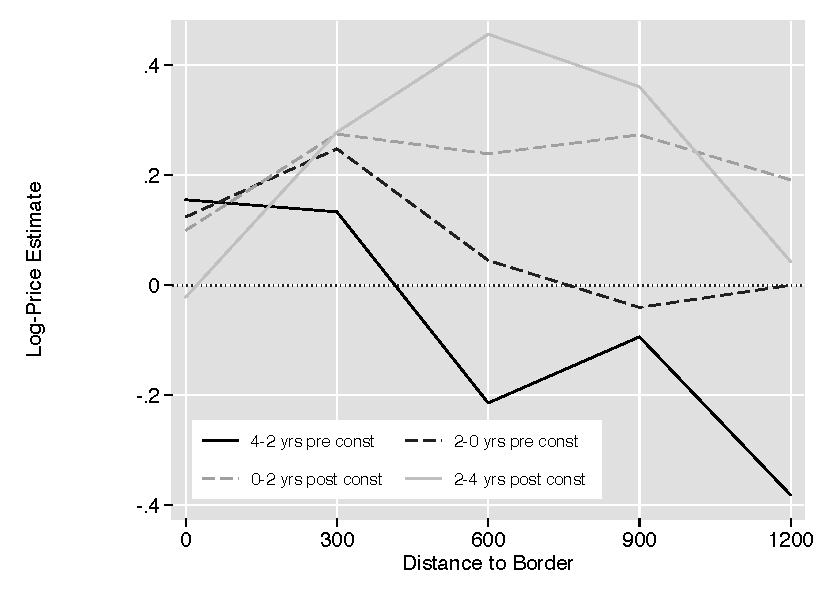
\includegraphics{figures/price_to_event_30.pdf}
% \end{figure}


\begin{table}
\small
\centering
\caption{Triple Difference Estimates on Purchase Frequencies}\label{table:priceDDD_het}
\vspace{-2mm}
\begin{tabular}{lCC}
\toprule
 & \small (1) & \small (2)  \\ \midrule 
 \textbf{All Projects} \\
 inside project      &      -0.007                   &      -0.007                   \\
                    &     (0.013)                   &     (0.013)                   \\[0.55em]
0-250m outside project &      -0.007                   &      -0.007                   \\
                    &     (0.005)                   &     (0.005)                   \\[0.5em]
250-500m outside project &      -0.007                   &      -0.007                   \\
                    &     (0.006)                   &     (0.006)                   \\[0.5em]
Lot Size Controls   &                               &  \checkmark                   \\
r2                  &        0.01                   &        0.01                   \\
N                   &   2,642,355                   &   2,642,355                   \\

 \midrule
\textbf{Greenfield} \\   inside project      &      -0.019                   &      -0.019                   \\
                    &     (0.024)                   &     (0.024)                   \\[0.01em]
0-250m outside project &      -0.007                   &      -0.007                   \\
                    &     (0.008)                   &     (0.008)                   \\[0.01em]
250-500m outside project &      -0.018\textsuperscript{c}&      -0.018\textsuperscript{c}\\
                    &     (0.009)                   &     (0.009)                   \\[0.8em]
\textbf{In-Situ Upgrading} \\   inside project      &       0.004                   &      -0.002                   \\
                    &     (0.009)                   &     (0.009)                   \\[0.01em]
0-250m outside project &      -0.013                   &      -0.012                   \\
                    &     (0.010)                   &     (0.010)                   \\[0.01em]
250-500m outside project &      -0.001                   &      -0.001                   \\
                    &     (0.011)                   &     (0.011)                   \\[0.8em]
\textbf{Other} \\   inside project      &       0.002                   &       0.002                   \\
                    &     (0.014)                   &     (0.014)                   \\[0.01em]
0-250m outside project &      -0.003                   &      -0.003                   \\
                    &     (0.008)                   &     (0.008)                   \\[0.01em]
250-500m outside project &      -0.001                   &      -0.001                   \\
                    &     (0.008)                   &     (0.008)                   \\[0.8em]
Lot Size Controls   &                               &  \checkmark                   \\
r2                  &        0.01                   &        0.01                   \\
N                   &   2,642,355                   &   2,642,355                   \\

\bottomrule
\multicolumn{3}{l}{\footnotesize Standard errors clustered at the project level in parenthesis.} \\
\multicolumn{3}{l}{ \textsuperscript{c} p$<$0.10,\textsuperscript{b} p$<$0.05,\textsuperscript{a} p$<$0.01 }
\end{tabular}
\end{table} 

% \begin{figure}
% 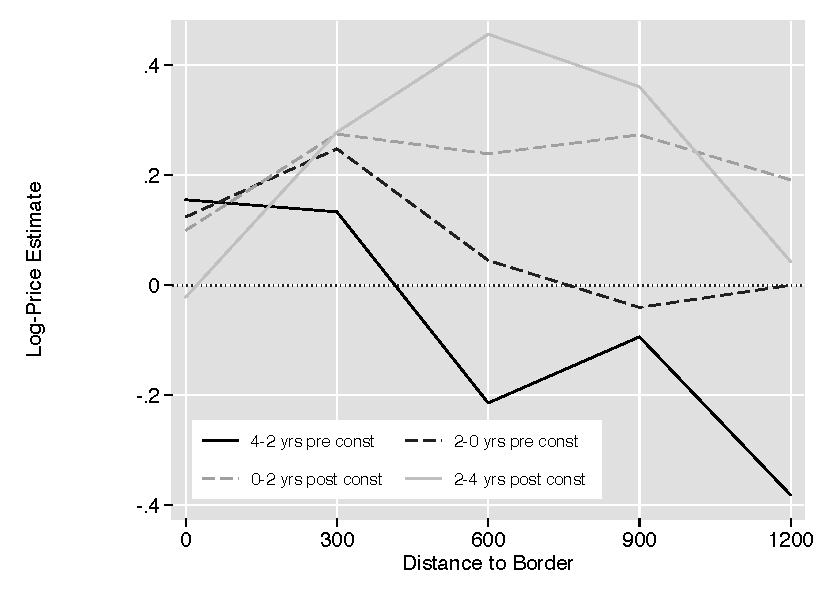
\includegraphics{figures/price_to_event_30.pdf}
% \end{figure}





\begin{table}
\caption{Effect of Housing Projects on Socio-demographics}
\label{table:sorting}
\small
\centering
%\caption{Census Composition Estimates }
\vspace{-2mm}
\begin{tabular}{lDDDDD}
\toprule
& \small (1) & \small (2) & \small (3) & \small (4)& \small (5)\\
& \small Age & \small P.O.B. not Gauteng & \small Unemployed & \small Years of Education & \small Monthly Income \\ \midrule 
\textbf{All Projects} \\inside project      &      -0.093                   &      -0.012                   &       0.023                   &       0.220\textsuperscript{c}&    1310.881\textsuperscript{b}\\
                    &     (0.310)                   &     (0.019)                   &     (0.021)                   &     (0.131)                   &   (603.631)                   \\[0.5em]
0-400m outside project &       0.346                   &      -0.010                   &       0.008                   &      -0.009                   &     585.976                   \\
                    &     (0.299)                   &     (0.017)                   &     (0.021)                   &     (0.098)                   &   (630.775)                   \\[0.5em]
400-800m outside project &      -0.218                   &       0.003                   &       0.017                   &       0.029                   &      49.181                   \\
                    &     (0.311)                   &     (0.016)                   &     (0.019)                   &     (0.107)                   &   (687.615)                   \\[0.5em]
R$^2$               &       0.630                   &       0.742                   &       0.481                   &       0.659                   &       0.604                   \\

\midrule
\textbf{Greenfield} \\   inside project      &      -0.871                   &       0.026                   &       0.074\textsuperscript{c}&      -0.274                   &    -969.577                   \\
                    &     (4.560)                   &     (0.049)                   &     (0.044)                   &     (0.255)                   &   (628.928)                   \\[0.01em]
0-400m outside project &       1.531                   &      -0.013                   &      -0.060                   &       0.227                   &    -652.224                   \\
                    &     (2.953)                   &     (0.045)                   &     (0.043)                   &     (0.209)                   &   (863.341)                   \\[0.01em]
400-800m outside project &       0.129                   &      -0.001                   &       0.054                   &      -0.206                   &   -2371.304\textsuperscript{b}\\
                    &     (3.003)                   &     (0.045)                   &     (0.058)                   &     (0.236)                   &  (1078.395)                   \\[0.8em] 
\textbf{In-Situ Upgrading} \\   inside project      &       0.922                   &       0.010                   &      -0.062\textsuperscript{c}&       0.331                   &     737.337                   \\
                    &     (2.198)                   &     (0.033)                   &     (0.037)                   &     (0.205)                   &   (861.316)                   \\[0.01em]
0-400m outside project &       1.429                   &      -0.072\textsuperscript{b}&       0.020                   &       0.248                   &     271.743                   \\
                    &     (1.671)                   &     (0.031)                   &     (0.029)                   &     (0.223)                   &   (895.312)                   \\[0.01em]
400-800m outside project &       3.372\textsuperscript{c}&      -0.047                   &       0.023                   &      -0.035                   &     230.140                   \\
                    &     (1.961)                   &     (0.030)                   &     (0.031)                   &     (0.175)                   &  (1047.239)                   \\[0.8em]
\textbf{Other} \\   inside project      &      -0.119                   &      -0.117\textsuperscript{a}&      -0.025                   &       0.804\textsuperscript{a}&    2929.182\textsuperscript{a}\\
                    &     (1.784)                   &     (0.032)                   &     (0.034)                   &     (0.182)                   &   (802.620)                   \\[0.01em]
0-400m outside project &      -1.329                   &       0.007                   &       0.031                   &      -0.096                   &    1287.094\textsuperscript{c}\\
                    &     (1.672)                   &     (0.024)                   &     (0.025)                   &     (0.134)                   &   (723.151)                   \\[0.01em]
400-800m outside project &       1.589                   &       0.018                   &       0.015                   &       0.200                   &    1276.535                   \\
                    &     (1.831)                   &     (0.023)                   &     (0.026)                   &     (0.163)                   &   (786.199)                   \\[0.8em]
Mean Outcome 2001   &       33.27                   &        0.37                   &        0.42                   &        8.61                   &    1,905.01                   \\
Mean Outcome 2011   &       28.30                   &        0.43                   &        0.33                   &        9.68                   &    4,505.16                   \\
R$^2$               &       0.203                   &       0.746                   &       0.481                   &       0.547                   &       0.581                   \\
N                   &      20,641                   &      12,729                   &      20,591                   &      20,637                   &      20,589                   \\

\bottomrule
\multicolumn{6}{l}{\footnotesize Standard errors clustered at the project level in parenthesis. \textsuperscript{c} p$<$0.10, \textsuperscript{b} p$<$0.05, \textsuperscript{a} p$<$0.01  }\\
\multicolumn{6}{l}{\footnotesize P.O.B. means ``place of birth.''  Monthly income is in Rands.}
\end{tabular}
\end{table}


\begin{table}
\caption{Effect of Housing Projects on Socio-demographics Two Diff-in-Diffs}
\label{table:sorting}
\small
\centering
%\caption{Census Composition Estimates }
\vspace{-2mm}
\begin{tabular}{lDDDDD}
\toprule
& \small (1) & \small (2) & \small (3) & \small (4)& \small (5)\\
& \small Age & \small P.O.B. not Gauteng & \small Unemployed & \small Years of Education & \small Monthly Income \\ \midrule 
\textbf{Constructed} \\ inside project      &       1.501\textsuperscript{b}&      -0.033\textsuperscript{a}&      -0.019\textsuperscript{b}&       0.102                   &   -1698.129\textsuperscript{a}\\
                    &     (0.685)                   &     (0.010)                   &     (0.009)                   &     (0.068)                   &   (161.833)                   \\[0.5em]
0-400m outside project &       0.609                   &      -0.007                   &      -0.005                   &      -0.084\textsuperscript{c}&    -928.554\textsuperscript{a}\\
                    &     (0.723)                   &     (0.009)                   &     (0.008)                   &     (0.049)                   &   (162.264)                   \\[0.5em]
400-800m outside project &       1.889\textsuperscript{b}&      -0.015\textsuperscript{c}&       0.001                   &      -0.131\textsuperscript{a}&    -761.819\textsuperscript{a}\\
                    &     (0.807)                   &     (0.008)                   &     (0.009)                   &     (0.048)                   &   (186.724)                   \\[0.5em]
\textbf{Unconstructed} \\ inside project      &      -1.345                   &       0.007                   &       0.013                   &      -0.593\textsuperscript{a}&   -3679.486\textsuperscript{a}\\
                    &     (3.549)                   &     (0.030)                   &     (0.033)                   &     (0.150)                   &   (573.724)                   \\[0.5em]
0-400m outside project &       1.490                   &      -0.008                   &      -0.033\textsuperscript{b}&      -0.081                   &   -1425.914\textsuperscript{a}\\
                    &     (1.201)                   &     (0.018)                   &     (0.017)                   &     (0.095)                   &   (519.742)                   \\[0.5em]
400-800m outside project &       0.567                   &      -0.007                   &      -0.029                   &      -0.332\textsuperscript{b}&   -2168.556\textsuperscript{a}\\
                    &     (1.590)                   &     (0.020)                   &     (0.019)                   &     (0.135)                   &   (668.486)                   \\[0.5em]
R$^2$               &       0.202                   &       0.742                   &       0.479                   &       0.542                   &       0.573                   \\

\midrule
\textbf{Treatment} \\ inside project      &       3.532                   &      -0.027                   &      -0.073\textsuperscript{b}&       0.650\textsuperscript{a}&     543.172                   \\
                    &     (3.492)                   &     (0.030)                   &     (0.033)                   &     (0.164)                   &   (398.871)                   \\[0.5em]
0-400m outside project &      -0.333                   &       0.011                   &      -0.008                   &      -0.098                   &   -1018.942\textsuperscript{a}\\
                    &     (1.127)                   &     (0.018)                   &     (0.016)                   &     (0.097)                   &   (290.688)                   \\[0.5em]
400-800m outside project &       1.954                   &       0.007                   &      -0.018                   &       0.110                   &    -427.453                   \\
                    &     (1.419)                   &     (0.019)                   &     (0.018)                   &     (0.132)                   &   (408.318)                   \\[0.5em]
\textbf{Control} \\ 800-1500m outside project&       0.595                   &       0.016                   &      -0.041\textsuperscript{a}&      -0.084                   &   -1424.311\textsuperscript{a}\\
                    &     (1.098)                   &     (0.010)                   &     (0.011)                   &     (0.057)                   &   (489.170)                   \\[0.5em]
R$^2$               &       0.202                   &       0.740                   &       0.466                   &       0.511                   &       0.563                   \\

\bottomrule
\multicolumn{6}{l}{\footnotesize Standard errors clustered at the project level in parenthesis. \textsuperscript{c} p$<$0.10, \textsuperscript{b} p$<$0.05, \textsuperscript{a} p$<$0.01  }\\
\multicolumn{6}{l}{\footnotesize P.O.B. means ``place of birth.''  Monthly income is in Rands.}
\end{tabular}
\end{table}



\end{document}


